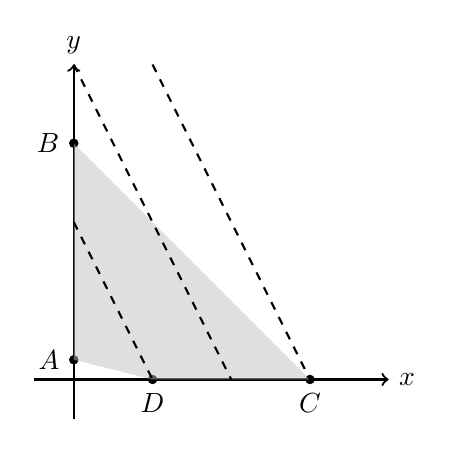
\begin{tikzpicture}
  \draw[->, thick] (-0.5, 0)--(4, 0) node[right]{$x$};
  \draw[->, thick] (0, -0.5)--(0, 4) node[above]{$y$};
  
  \node[
    circle,
    draw=black,
    fill=black,
    inner sep=0pt,
    minimum size=3pt,
    label=below:{$D$}
  ] (d) at (1, 0) {};

  \node[
    circle,
    draw=black,
    fill=black,
    inner sep=0pt,
    minimum size=3pt,
    label=below:{$C$}
  ] (c) at (3, 0) {};
  \node[
    circle,
    draw=black,
    fill=black,
    inner sep=0pt,
    minimum size=3pt,
    label=left:{$B$}
  ] (b) at (0, 3) {};
  \node[
    circle,
    draw=black,
    fill=black,
    inner sep=0pt,
    minimum size=3pt,
    label=left:{$A$}
  ] (a) at (0, 0.25) {};
  
  \fill[
    opacity=0.5,
    gray!50
  ] (1, 0) -- (3, 0) -- (0, 3) -- (0, 0.25) -- cycle;
  
  \draw[dashed, thick] (0, 2) -- (1, 0);
  \draw[dashed, thick] (0, 4) -- (2, 0);
  \draw[dashed, thick] (1, 4) -- (3, 0);
 
\end{tikzpicture}
